\documentclass[12pt,a4paper]{article}
\usepackage[latin1]{inputenc}
\usepackage{amsmath}
\usepackage[T1]{fontenc}
\usepackage{palatino}
\usepackage{algorithm2e}
\usepackage{algorithmic}
\usepackage{hyperref}
\usepackage{amssymb}
\usepackage{graphicx}
\author{Alexandros-Panagiotis Oikonomou}
\setlength{\parindent}{15pt}
\begin{document}
\begin{titlepage}
\begin{center}
\begin{LARGE}
Electronics and Computer Science
Faculty of Physical and Applied Sciences
University of Southampton 
\end{LARGE}
\\[2cm]
\begin{large}
Alexandros-Pana Oikonomou
\\
1$^{st}$ May 2013
\\[2cm]
Solving the Conjugate Gradient Method in a SpiNNaker Machine
\\[3.5cm]
Project Supervisor: Jeff Reeve
\\Second Examiner: Marcus Breede
\\[3.5cm]
A project report submitted for the award of
\\BSc Computer Science
\end{large}
\end{center}
\end{titlepage}
\section*{Abstract}
\pagenumbering{gobble}
SpiNNaker is an asynchronous, event-driven parallel architecture designed to simulate
the human brain. It has been designed to operate as a large scale neural network in
real-time using a System-on-Chip multi core system. Its architecture is different from
usual parallel computers, since cores use spikes to communicate with each other. That
way usual pitfalls of parallel computing, such as race conditions and deadlocks are
avoided. So far the most prominent uses of this architecture have been in
neuroscience and robotics. The aim of this project is to put into use SpiNNaker's
architecture and bring it closer to classic computer science problems, while solving
them optimally. The given algorithm to solve in this project is the conjugate gradient
method, an iterative way of solving systems linear equations. The algorithm successfully runs on the simulator and reduces the time complexity of the most expensive operations of the algorithm.
\newpage
\tableofcontents
\newpage
\section*{Acknowledgments and Statement of Originality}
I would like to thank my supervisor Jeff Reeve for his help and support throughout this project.
\newpage
\section{Introduction}
\pagenumbering{arabic}
\subsection{Aim}
The aim of this project is to correctly solve the Conjugate Gradient Method\cite{hestenes1952methods} on a SpiNNaker chip, thus using the massive parallelism that this machine offers to reduce the time complexity of the aforementioned algorithm. This is accomplished by reducing the time complexity of the most expensive operations of the algorithm which are matrix-vector multiplication and the scalar product of vectors. The complexity is reduced dramatically, due to the abundant number of cores provided from the architecture. This report explains this project and its constituents, any background research done to launch this project, along with designe and implementation choices.
\subsection{Reasons and Justification}
\indent
SpiNNaker is an architecture inspired by the biology of the human brain. Its optimal configuration has over a million cores\cite{navaridas2009understanding}, which have mainly been used to simulate the neurons of the human brain and in robotics.

However little work had been done into using the SpiNNaker architecture to solve classic computer science problems. That is why a problem such as the Conjugate Gradient Method had been proposed, which is a very common solution to optimization problems. In addition to that, the SpiNNaker architecture offers new parallel programming paradigms, that escape some common parallel programming pitfalls such as race conditions, deadlocks, mutual exclusion etc\cite{sharp2011event}.
\subsection{Overview}
Give a brief overveiw of what each section contatins
\newpage
\section{Background}
\subsection{The neuron}
To make the explanation of the SpiNNaker architecture easier, the design from which the SpiNNaker chip was inspired will be outlined. This is no other than the human neuron.

The human neuron is an electrically excitable cell that processes and transmits information through electrical and chemical signals. Its basic costitutes are the the soma, the dendrites and the axon. The soma is the body of the neuron. A dendrite receives signals from the soma of the neuron that it belongs to or other neurons. The dendrite extends for hundreds of micrometers and branches multiple times, thus forming a dendritic tree, which connects with other neurons axons. The axon is used to transmit signals to other neurons and it extends from the soma of the neuron to a dendrite. All human neurons have only one axon. Given the above analysis the dendrites could be described as the inputs of a neuron
\\[0.5cm]
\begin{figure}[h!]
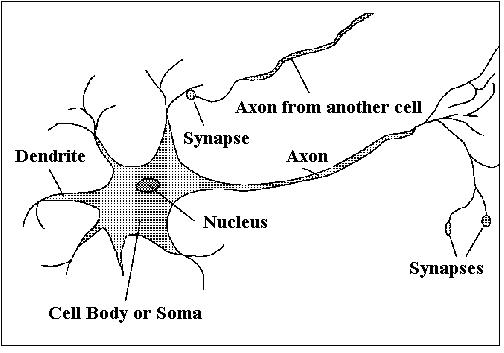
\includegraphics[width=300pt,height=200pt,scale=2]{Pics/neuron.jpg}
\centering
\caption{A neuron}
\end{figure}

One of the most important parts of the neuron structure is the synapse. The synapse is the contact between the axon of a neuron and the dendrite or the soma of another. It is where a information from one neuron is transmitted to the other. When a set of neurons are connected with each other through synapses, then they create a neural network.

Finally, the communication between neurons is accomplihed through spikes, which are either chemichal or electrical\cite{gerstner2002spiking}.

Given the terms in this section, the name of the SpiNNaker chip is detuctable. It stands for Spi(king)N(eural)N(etwork) architecture.
\subsection{The SpiNNaker architecture}
As mentioned before the SpiNNaker architecture is inspired by the biology of the brain, and more specifically, neurons. However, its architecture is not constrained by the biology of the brain, but many techniques to speed up computations are used. It differs from other supercomputers, which  usually have a lot of strong processors with slow network capabilities. The design of the architecture was made with having as priority two concerns. The first one being MIPS(millions of instructions per-second) per mm$^2$. Namely how many instructions can be performed in an area of silicon. The second one was MIPS per watt, which means how many instructions per second can be performed given a fixed amount of energy. Its most optimal configuration will use a million cores and will be able to simulate over a billion neurons\cite{furber2007neural}.
\subsubsection {SpiNNaker chip Overview}
The heart of the SpiNNaker architecture is the SpiNNaker chip. Its main components are 18 identical ARM cores that run at around 100Mhz each, a router, a system NoC(Network-on-Chip) which connects to the router of the chip and a 128 MB SDRAM. At startup, in each chip a processor is selected to act as a Monitor processor, with the functionality of performing the management of the given chip's system. The remaining ARM cores perform the calculations for the given problem, with the exception of one which is reserved as a spare, in the emergency of another core having a malfunction\cite{furber2007neural}. Each core has the ability to hold 32KB of instructions and 64KB of data. Since this is not enough space, all other data is saved in the SDRAM which can hold up to 1GB of data\cite{navaridas2009understanding}.
\begin{figure}[h!]
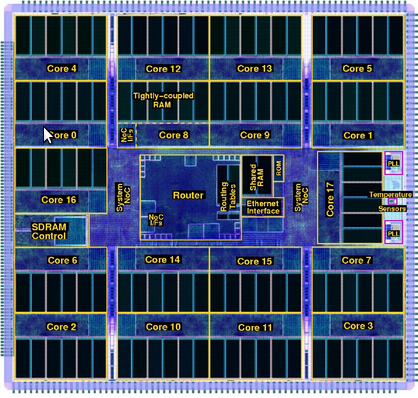
\includegraphics[width=250pt,height=150pt,scale=2]{Pics/chip.png}
\centering
\caption{The SpiNNaker chip\cite{spinnweb}}
\end{figure}
\subsubsection{The router}
As mentioned before the architecture supports low-delay communication, with less powerful processors, than those used in most supercomputers. To accomplish that, the system uses asynchronous multicast packets to communicate between cores. This is done through the router which exists in each chip.

The router exists as the part of the NoC and its primary role is to direct packets that arrive and packets that are sent or need to be forwarded. The router has 20 ports for the ARM cores that are located in the given chip and is able to forward one packet at a time. The router works faster than a transmission port, which results into the router being most of the time lightly used. It is designed to support point-to-point communication, using small packets. Using multicast packets helps reduce the amount of packets that exist in any givne moment in the network. To help with that, the architecture supports default routing, which means that some connections do not need to be in some routing tables for them to be forwarded to their eventual destination. This concept will be explained in the next section.

The functionality of the router is pretty simple. When a packet arrives from the input port, then the router will try to send it to an output port. If there is a problem during transmission, then the router will keep trying to send it and after a while it will try the emergency route(also explained in the next section). If the emergency route still does not work and an amount of time is passed, then the packet will be dropped. To help with that, each packet has the time it was transmitted in their header.

\begin{figure}[h!]
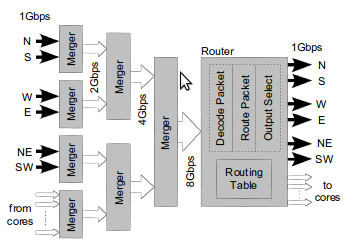
\includegraphics[width=250pt,height=150pt,scale=2]{Pics/router.png}
\centering
\caption{The router\cite{navaridas2009understanding}}
\end{figure}
To further understand this concept, the topology of the system needs to be considered.
\subsubsection{Topology}
In order to have a million cores available for processing a number of SpiNNaker chips need to get connected and work efficiently as an architecture. To reach that goal an effective topology is important.
\begin{figure}[h!]
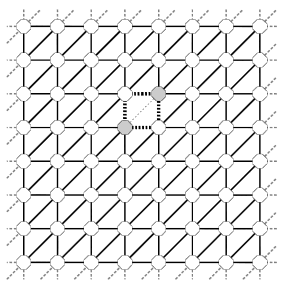
\includegraphics[width=250pt,height=250pt,scale=2]{Pics/topology.png}
\centering
\caption{
\emph{The SpiNNaker topology\cite{navaridas2009understanding}. This is an example of what an 8x8 would look like.Each circle is a SpiNNake chip and the lines between them are the connectivity.}}
\end{figure}
\vspace{20pt}
Considering Figure 4, it is visible that the topology is viewed by the system as a 2D mesh, with chips having a specific amount of neighbours and specific connections. Any chip is able to communicate directly to 6 other chips. This is also depicted in Figure 3, where the positions of these chips are shown. In general each chip directly communicates with chips that are North, South, West, East ,NorthEast, and Southwest of its respective position. This however does not apply for chips that are in the perimeter of the mesh, since they in some of the positions described above chips will not exist\cite{furber2012overview}. 

Returning now to the default routhing mentioned in the previous section, if a packet arrives to a router, and the router does not have an entry for it, a then it will be forwarded to the chip opposite to the one it came from. For example, if a packet comes from the East and the aforementioned condition is met, then it will be forwarded to the West. This helps reduce the size of the routing tables in each chip\cite{khan2008spinnaker}.

In addition to the default routing, the topology also provides for two-hop routes aming neighbor chips, as shown in Figure 4. These routes are named emergency routes and their functionality is to bypass any faulty connections that might exist between connections\cite{navaridas2009understanding}\cite{plana2007gals}.

\subsubsection{Packets}
The packets used in the architecture are all multicast packets. They asynchronous and relatively small. Having multicast packets means that one packet might have many different destinations, and with potentially a million cores, they can have thousands of destinations. For that reason, the packets do not contain the destination(s) they are supposed to reach, but rather only the source. Their size is of around 40 or 70 bits and their transmission is done completely by the hardware of the system, thus having high bandwidth\cite{spinnweb}\cite{navaridas2009understanding}. It is also notable that, when simulating a billion neurons, unique addresses are needed to acknowledge them. Hence 32-bit addresses are used to represent items in the cores. In this architecture, the main packets used can be divided in two types.
\begin{itemize}
\item Multicast packets(Type 0). Consists of 32-bit source address, 8 bits of control and 32-bit payload. These types of packets are delivered to processors and usually would contain information for computation
\item Point-to-point packets(Type 1). Consists of 16-bit source \emph{chip} address, 16-bit target \emph{chip} address, 8-bit control payload and 32-bit payload. It is a command/control packet and is used when the Monitor Processor communicates with the target chip\cite{docfile}
\end{itemize}

in this project mainly the Type 0 packets have been used.
\subsubsection{Routing Tables}
A mention of the routing tables is also important in understanding the architecture. Optimally, one would want for all cores to communicate with all the other cores in the system. However, that would be impractical, since the data structure that would exist in the routing table would have to be enormous.

This architecture supports routing tables of 1024 entries. Each entry is of 32-bit size, since it needs to hold addresses for the routing. The nature the most siginificant bit of the source is written determines if a particular packet is for distributing locally to the cores, or if it should be linked and forwarded to other chips\cite{docfile}.
\subsubsection{Bandwidth}
Having talked about how the architecture works, it would be a good point to talk about the bandwidth bisection that it offers. Assuming the optimal configuration of the SpiNNaker architecture with a million cores, then it is safe to assume that the number of chips that will be used, would be around 63K. If we would split the topology in two then the optimal goal would be to have all the neurons of one half connected to at least one neuron in the other half. That way, the bandwidth in the border would be 6.4G packets/sec. Another safe assumption is that the 2D mesh for this machine would be 256x256. Given that each node should carry 25M packets/sec\cite{docfile}\cite{navaridas2009understanding}.
\newpage
\subsection{Software}
There is a lot that comes when trying to run any kind of software in a SpiNNaker board. The basic devices that are used to run software are three.
\begin{itemize}
\item Host Machine, which is mainly used for input and output, and it is the component that the user interacts with to start an application
\item Monitor Cores. This is the same Monitor core that was discussed previously. Its main use is monitoring and managing the system and the application cores. One of them also communicates with the host, in order to start up the program.
\item Application Cores, which are used to carry out the computation of the application.\cite{furber2012overview}
\end{itemize}

At this point it is noteworthy to mention that the programming model of the machine is event-driven, meaning computations occur when specific events take place. More on that will be covered in late sections
\subsubsection{Startup}
In order to do the startup the devices mentioned above some kind of software needs to be used. For the Host machine to interact with the main Monitor Core \emph{ybug} is used. It is also used to start applications. Ofcourse ybug does not communicate only with the hardware of the monitor core. There is another software called \emph{scamp}, that works on top of the Monitor Core. It interacts with the ybug and the \emph{sark}, which is a software that is used by the application cores. Sark lets the user to manipulate some hardware parts of a SpiNNaker chip.\cite{spinnweb}
\subsubsection{Local Data Structures}
Before the application starts running, some other applications need to be comlpeted first. These include finding the state of the machine, finding a communications tree and sketching out the point-to-point tables.

\paragraph{The state of the machine}
To discover the state of the machine, each chip checks its cores and the connections between them to check whether any broken links exist. How the algorithm works is that firstly a root node is selected and is marked with a Request(R) token. Each time a core has a R token it sends an Acknowledge(A) label to all the incoming ports. If the labeling is successful, then that incoming port is deemed Good. Otherwise it tries to send an R token to that port and it marks it as Broken\cite{jefflec}.
\paragraph{Building a communications tree}
In order to build a communication tree a breadth first tree traversal is used. To achieve that firstly a root node is selected and given the token Forward(F). The root node speaks to neighbour nodes and after giving them the label Child it says to them to also send F tokens to all their neighbours, thus making them parents. Once there are not any more unlabelled nodes, the nodes are instructed to return a Backwards(B) token to their parent nodes. That way the system becomes aware of which nodes communicate with each other. If by any chance two nodes send to each other a B token through the same port, then that port is deemed non communicational and is labelled Unused. The reason for that is to avoid any loops in the system\cite{jefflec}.
\paragraph{Creating the P2P Tables}
In order to know to which nodes a packet needs to be sent, the nodes need an ID. Point-to-Point tables are used to list the ID's of nodes, so it knows which port it should follow. At first all nodes are undefined(U). If we were to find the entry for one undefined node then the table would mark its own incoming port and send its port to all other ports.  That way all the other chips in the board would know what port to use to communicate with that node. For the nodes that are on the same chip with that node............If that is done for the all of the nodes in the system, then the P2P table is built\cite{jefflec}. 

\subsubsection{Program Loading}
In order to begin running a program some input needs to be provided to the system. The way this is currently done is by using the static model. With the static model the network topology, the connections between nodes and the allocation of the hardware is provided explicitely and externally by the user, before the execution of the program. Moreover, data and additional execution information needs to be defined before the program is loaded in the machine. This information is read from an external machine and written again in a fashion that is readable by the machine. This is usually done through binary files. the Host starts the execution of the program, after the 'readable' version is has been loaded to the machine. When the program terminates, or the user wishes to terminate it, then the Host issues a halt command that stops all operations\cite{docfile}.

There is an additional model for loading data in the system called the dynamic model, which would enable the machine to figure the network topology by itself, while running the application. However, this kind of a model is still in low stages\cite{docfile}.
\subsubsection{Event Handling}
As mentioned before the SpiNNaker architecture's programming model is event-driven. For a function to be executed by a an application core, a certain event needs to occur beforehands. In the context of SpiNNaker there are three events that can cause a function to run.
\begin{itemize}
\item Delivery of a packet.
\item Completion of a DMA transfer.
\item After a time interval.
\end{itemize}
Each of these bullet points qualifies as an event. The programmer cannot really control when these specific events will take place(except in the case of the time interval). What the programmer can control is the what happens when such an event occurs. The functions, in this context referred as callbacks, are written by the programmers, which after a specific event occurs, are given a priority with the kernel(sark). 
\begin{figure}[h!]
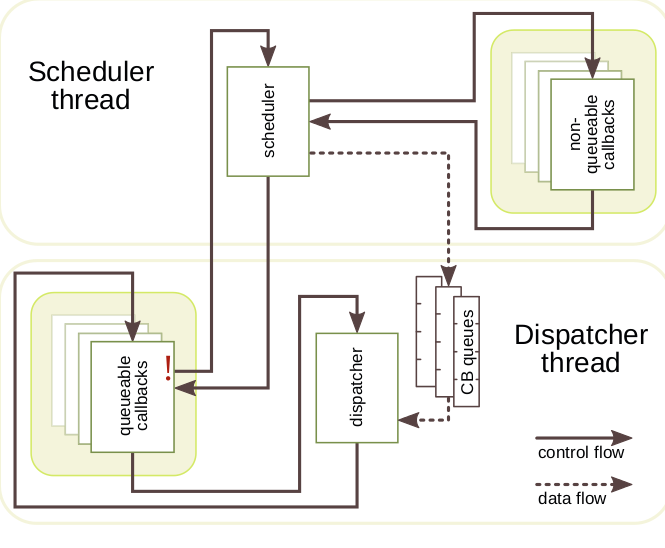
\includegraphics[width=250pt,height=150pt,scale=2]{Pics/event-handling.png}
\centering
\caption{Event-handling. The control and data flow is shown\cite{sharp2011event}}
\end{figure}
The types of callbacks can be seperated in two categories. Queueable and non-queueable. In the case of a non-queuable callback, the callback is executed immediately by the system, having the top priority of execution. A queueable callback, which is most common, will be put on an execution queue along with other queueable callbacks. In the case that the queue empties, no callbacks will be executed. It will continue executing callbacks when another event occurs at some point\cite{sharp2011event}\cite{rast2012managing}. 
	
\subsection{Notable work using the SpiNNaker architecture}
Most of the notable work done in SpiNNaker machines is simulation of neurons. Each time different sets of neurons would be used to be simulated. An example would be simulating the neurons of the retina, so as to make it possible for a robot to calculate its place\cite{davies2010interfacing}. Another one would be simulating thousands of spiking neurons using four million synapses\cite{sharp2012power}. Another interesting application would be teaching temporal sequences  of discrete symbols, thus making fast and accurate predictions of new sequnces\cite{bose2005spiking}.
Most of the notable work done in SpiNNaker machines is simulation of neurons. e
\subsection{Conjugate Gradient Method}
The conjugate gradient method is an algorithm for the numerical solution of systems of linear eqations of the type Ax=b, those whose matrix is symmetric and positive definite. 

A \emph{symmetric} matrix is a matrix which is equal to its transpose. If A is a symmetric matrix then A=A$^T$. The entries of the matrix are symmetric with respect to the main diagonal, so if an element of the matrix A is a, then a$_{ij}$=a$_{ji}$. 
A \emph{positive definite} matrix M is a matrix which when multipled by any non-zero vector z and its transpose z$^T$, is always positive. In short the relationship that needs to be satisfied is zMz$^T$>0

It is an iterative method, which means it can be applied to sparse systems. A \emph{sparse matrix} is a matrix which is populated primirily with zeros. Its opposite would be a \emph{dense matrix}. It was developed by Magnus Hestenes and Eduard Stiefel and can be used to solve optimization problems\cite{press2007numerical}.
\subsubsection{The quadratic form}
In order to explain why the Conjugate Gradient Method can solve problems whose matrix is positive-definite and symmetric an explanation of the quadratic form needs to be presented.
\begin{center}
\begin{equation}
f(x)=\frac{1}{2}x^TAx-b^T+c
\end{equation}
\end{center}

The gradient $\nabla f(x)$ of the quadratic form is a vector field that points in the direction of the greatest increase of $f(x)$. If we were to take into account the i$^{th}$ component of $\nabla f$, then.
\begin{equation}
\begin{split}
f(x+\psi e_i)= \frac{1}{2} (x+\psi e_i)^TA(x+\psi e_i)-b^T(x+\psi e_i)+c\\
= \frac{1}{2} (x^TAx+\psi e^T_iAx +x^TA\psi e_i)-b^T(x+\psi e_i)+c
\end{split}
\end{equation}
Note that e$_i$ is the error affiliated with taking the i$^{th}$ component of $\nabla f$. Now from the definition of a derivative $f(x)$=$\frac{f(a+h)-f(a)}{h}$ and (2) we have.
\begin{equation}
\frac{f(x+\psi e_i)-f(x)}{\psi}=\frac{\frac{1}{2}(\psi e^T_iAx+x^TA\psi e_i)-\psi e^T_ib}{\psi}
\end{equation}
(3) is the same as the i$^{th}$ component of $\frac{1}{2}$(Ax+A$^T$x)-b
So we have
\begin{equation}
\nabla f =\frac{1}{2}A^Tx+\frac{1}{2}Ax-b
\end{equation}
But if A is symmetric, then it is obvious that we have $Ax=b$ at the minimum of $f$. In addition if A is positive negative then $f$ is concave up.
\subsubsection{Conjugate Gradients}
As mentioned before the matrix A must be symmetric and positive definite for the Conjugate Gradient Method to work. Given a quadratic function 
as defined in (1), then it turns out that $-\nabla f=b-Ax=r$.

The CGM, as well as most optimization methods(for example the method of the Steepest Descent\cite{rosenbloom1956method}), look towards a specific direction everytime they are to move to a correct position and try to look for the best step given their gradient and direction
\begin{equation}
x_{k+1} = x_k + \alpha p_k
\end{equation}
Given (5), $\alpha$ can be deduced from the fact that $e_{k+1}$(the error vector of each iteration) must be orthogonal to p$_k$,  which also means that p$_k$ will never be met again as the solution progresses. Using this we can dedcuce
\begin{equation}
\begin{split}
p^T_ke_{k+1}=0\\
p^T_k(e_k+\alpha p_k)=0\\
\alpha = -\frac{p^T_ke_k}{p^T_kp_k}
\end{split}
\end{equation}

The equation at (6) however is not solvable. The value of $e_k$ is needed in each iteration, which is not computable at that time. To help with that the search directions in each iteration($p_k$) is defined as A-orthogonal in respect to the matrix A, instead of just orthogonal. The definition of A-orthogonal vectors is, given a matrix A, then:
\begin{equation}
p^T_kAp_k=0
\end{equation}
Given (7), $e_{k+1}$ and $p_k$ must be A-orthogonal. If we wish to find the optimal value for $\alpha$,then the gradient must be set to 0. This leads to the following equation.
\begin{equation}
0=\frac{d}{d\alpha}f(x_{k+1})=\nabla f(x_{k+1})^T\frac{d}{d\alpha}x_{k+1} = -r^T_{k+1}\frac{d}{d\alpha}(x_k + \alpha p_k) = -r^T_{k+1}p_k=p^T_kAe_{k+1}
\end{equation}
From (6),(7) the equation for $\alpha$ when $e_k$ and $p_k$ are A-orthogonal is
\begin{equation}
\begin{split}
\alpha =-\frac{p^T_kAe_k}{p^T_kAp_k}\\
=\frac{p^T_kr_k}{p^T_kAp_k}
\end{split}
\end{equation}

Another important equation that comes from analysing the error term is
\begin{equation}
p^T_kr_k=u^T_kr_k
\end{equation}

In (10) $u^T_k$ are u vectors that span the vector subspace of the vector field of $p_k$. They are also orthogonal to $r_k$ and $u_{k+1}$ is also orthogonal to all the previous $u$ vectors.

Using (9) and (10) we are able to reach a more accurate value for $\alpha$
\begin{equation}
\alpha = \frac{r^T_kr_k}{p^T_kAp_k}
\end{equation}

Using (9) and (10) and a Gram-Schmidt conjugation we are able to reach and a value for $\beta$
\begin{equation}
\beta = \frac{r^T_{k+1}r_{k+1}}{r^T_kr_k}
\end{equation}
\newpage\cite{rast2012managing}
\subsubsection{The algorithm}
Combining the optimal value of $\alpha$(8) and $\beta$(9) and a good step direction for p$_k$ the Conjugate Gradient Method is formed as follows
\\
\begin{algorithmic}
\STATE r$_0$=b-Ax$_0$
\STATE p$_0$=r$_0$
\STATE k=0
\FOR{k to 1000000}
\STATE $\alpha_k=\frac{r_k ^T*r_k}{p_k ^T*A*p_k}$
\STATE x$_{k+1}$=x$_k$+$\alpha_k$*p$_k$
\STATE r$_{k+1}$=r$_k$-$\alpha_k$*p$_k$*A
\IF{r$_{k+1}^T$*r$_{k+1}$ is small enough}
\STATE break
\ENDIF
\STATE $\beta_k=\frac{r_{k+1} ^T*r_{k+1}}{r_k ^T*r_k}$
\STATE p$_{k+1}$=r$_{k+1}$+$\beta_k$*p$_k$
\STATE k=k+1
\ENDFOR
\end{algorithmic}
\vspace{20pt}
Some notes that can be made about this algorithm are that the axis is defined by the eigenvectors of A and that the algorithm takes a conjugate step closest to $r$. Finally, the algorithm guarantees convergeance in at most n steps.\cite{press2007numerical}\cite{shewchuk1994introduction}\cite{cgm2009lec}

Ofcourse there is an error that exists in every step, as mentioned before, but it is minimized in each iteration. The error function would be:
\begin{equation}
\begin{vmatrix}
e_k
\end{vmatrix}
\leq 2(\frac{\sqrt{\kappa}-1}{\sqrt{\kappa}+1})^k
\begin{vmatrix}
e_0
\end{vmatrix}_A
\end{equation}

In Equation 9 $\kappa$ is the condition number.

Another interesting applicatoin of the Conjugate Gradient Method is that you can apply precondition on it in order to find the solution faster. However, preconditioning is outside of the scope of this project, since it adds a lot more calculation and would need a less general solution.
\subsubsection{Parallel solutions of the CGM}

Some parallel implementations of the CGM use blocks of the input vectors and matrix and assign them carefully to specific cores, thus letting each core produce output that will be used in the next iteration. These kinds of solutions work better with vector processors, since it allows a processor to complete large vector operations. Depending on how many processors a machine has, parts of the algorithm can continue being sliced to blocks, until the optimal implementation is reached\cite{o1987parallel}.

Some other parallel implementations try to use more specific preconditionings to achieve faster results, but again for the parallel part, they split the input into blocks to distribute it to various cores\cite{adams1985m}\cite{adams1983m}. 

One of the most interesting implementations of the CGM, suggests an improved algorithm named ICGS(Improved Conjugate Gradient Squared), which is based in another already altered version of the CGM\cite{maheswaran1999mcgs}. This implementation computes all vector-matrix  multiplications and inner products concurrently, for each iteration. The communication time between these operations and vector updates has been organised efficiently, so that global communication drops significantly, thus dropping the run time of the algorithm as well\cite{yang2001improved}.

Finally, there are many recent implementations which have used GPU's in order to solve the Conjugate Gradient Method efficiently. These pieces of work use CUDA and various other techniques to accomplish their goal, with some very good results. Ofcourse different GPU models are used, but that just enhances the generality of the solution. Generally though,as is for most parallel implementations of the CGM, the most used technique is reducing the time it takes to compute the matrix-vector multiplication and inner products, thus reducing the time of the algorithm overall\cite{galiano2012gpu}\cite{wozniak2010parallel}.
\section{Design}
As it was stated in the introduction the purpose of this project was to significantly reduce the time that the CGM takes to run, by reducing the time complexity of its most expensive computations. These computations were matrix-vector multplication and inner-product. In this section the basic communication, the matrix-vector multiplication and the flow of the program is considered.

Throughout this section, each core is going to be referred as a node, so as to think the system as a graph. This might help visualising the problem.
\subsection{Basic communication}
Using the massive parallelism that the SpiNNaker architecture provides with over a million cores, it was a clear step that each element of the input matrix(A) and vectors(b,r) would be put into a different node. 
\begin{figure}[h!]
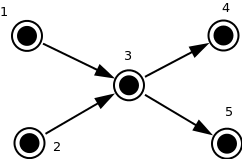
\includegraphics[width=250pt,height=150pt,scale=2]{Pics/basic.png}
\centering
\caption{Basic communication between nodes.}
\end{figure}
Considering that choice, it is easy to see that each node would need to receive and send spikes to different node at each time in the same fashion that Figure 6 shows. In that figure node 3 receives packets from nodes 1 and 2 and after some manipulation of the incoming data it sends its results to nodes 4,5. 

If this model is to be used each computation would be completed atomically and if only one computation is needed every time then the complexity at each core would be $O(1)$.
\subsection{Matrix-Vector Multiplication}
Using the above model a matrix-vector multiplication would look like Figure 7. 
\begin{figure}[h!]
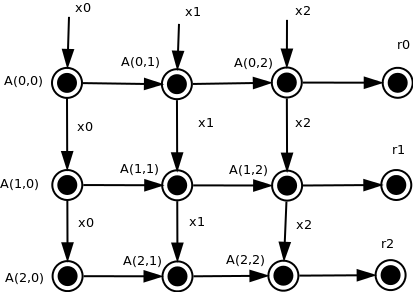
\includegraphics[width=250pt,height=150pt,scale=2]{Pics/mat0mult.png}
\centering
\caption{Matrix-vector multiplicatio for A*x.}
\end{figure}

In Figure 7 the first matrix-vector multiplication of the algorithm is used($Ax=r$) to display the general overview of this operation in the example of a 3x3 matrix and a 3x1 vector. To do the calculation, the $x$-nodes send a packet with their value to the respective $A$-nodes, where the multiplication part is completed. The $x$-nodes know to which $A$-nodes they should send based on the connections that was provided beforehands by the user. The column of the element in the matrix is considered to identify which $x$ nodes should be received by the $A$-nodes. Even though the figure shows that $A$-nodes send their value to next $A$-node in the column, the graph means to show that the $x$-nodes are the ones that are sent. The figure is shown that way for means of clarity. The same applies for when a $A$-node, after having completed the multiplication, sends the result to its respective $r$-node. Each time a packet arrives in the $r$-node an addition occurs, so as to complete the additive part of the multiplication. 

Given the figure above, it is clear that the multiplication in each $A$-node is done in $O(1)$. The same applies for the addition in the $r$-nodes, since there is some delay from the time the packet is sent and it arrives. Considering the communication tree built and discussed in section 2.3.2, the overall time-complexity for a matrix-vector multiplication to occur is $O(1)+log_2(N)+O(1)$. However, this is an optimal time-complexity that requires only one computation in each node. In practice, the complexity is larger.
\subsection{TT Format}
\subsection{Flow of Program}
\subsection{Constant nodes}
\newpage
\bibliographystyle{plain}
\bibliography{ref.bib}
\cite{navaridas2009understanding}
\cite{sharp2012power}
\cite{davies2010interfacing}
\cite{sharp2011event}
\cite{gerstner2002spiking}
\cite{press2007numerical}
\cite{shewchuk1994introduction}
\cite{cgm2009lec}
\cite{o1987parallel}
\cite{adams1985m}
\cite{maheswaran1999mcgs}
\cite{yang2001improved}
\cite{adams1983m}
\cite{galiano2012gpu}
\cite{wozniak2010parallel}
\cite{hestenes1952methods}
\cite{rosenbloom1956method}
\cite{furber2007neural}
\cite{spinnweb}
\cite{khan2008spinnaker}
\cite{docfile}
\cite{plana2007gals}
\cite{furber2012overview}
\cite{bose2005spiking}
\cite{jefflec}
\cite{rast2012managing}
\end{document}